% Main body with filler text
\begin{figure*}[t!]
    \centering
    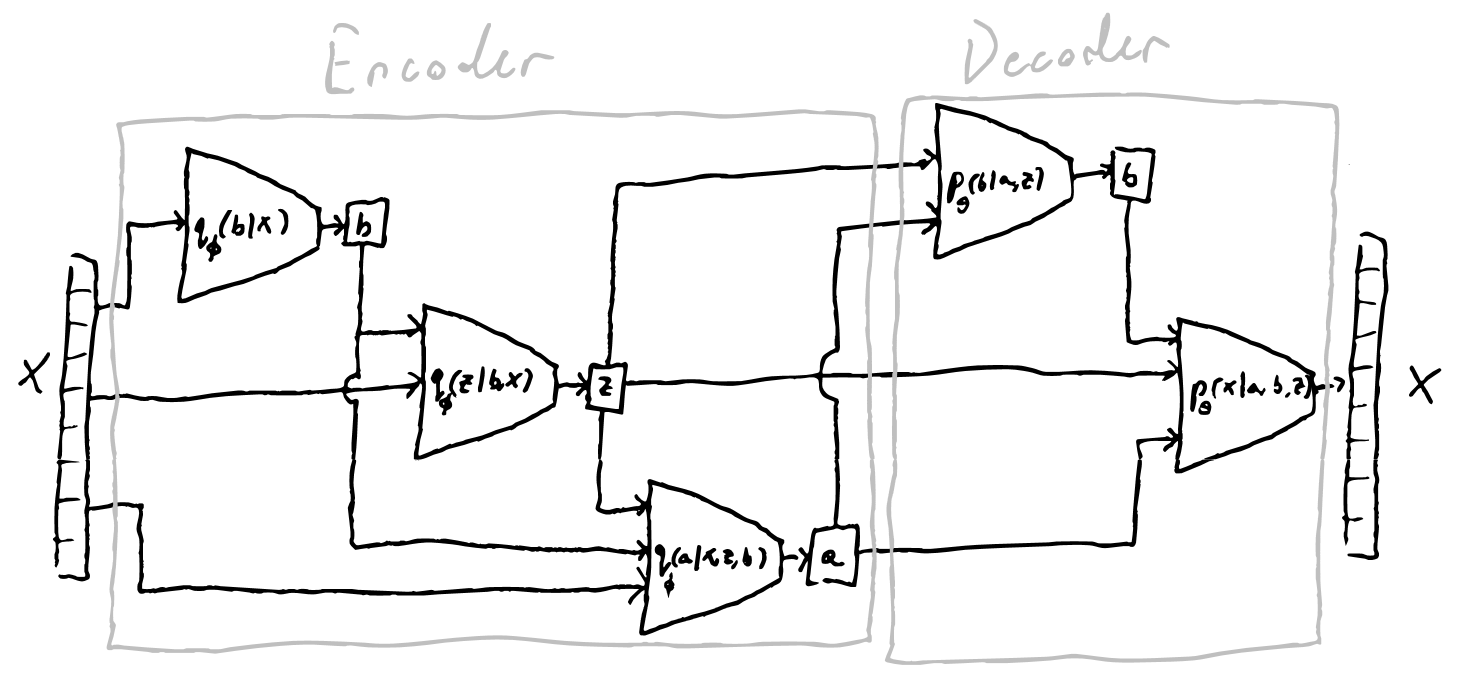
\includegraphics[width=\textwidth]{figures/model_sketch.png}
    \caption{\textbf{Rough sketch, to be redone using tikz.} Schematic illustrating the component distributions used in the SDGM, the base architecture of the \textsc{PhotoVAEz} model. The encoder takes as input the vector of photometric measurements $\mathbf{x}$ and consists of the variational distributions over the auxilliary latent space $\mathbf{b}$, the latent space $\mathbf{a}$ and $\log(z)$. The decoder takes as input samples from the encoder distributions and consists of the distributions over the auxilliary latent space $\mathbf{b}$ and the input photometry $\mathbf{x}$. All distributions shown are parameterized using neural networks.}
    \label{fig:sketch}
\end{figure*}

\section{\textsc{PhotoVAEz}}
\label{sec:methods}

% \subsection{Variational Autoencoders}
% \label{subsec:vae}

% A standard VAE, outlined in Fig. \textcolor{red}{[INSERT FIG]}, is composed of two neural networks referred to as the \textit{encoder} and the \textit{decoder}. The encoder is parameterized by $\boldsymbol{\theta}$ and maps an input vector $\mathbf{x}$ to a distribution over the lower-dimensional latent space, $q_{\boldsymbol{\theta}}(\mathbf{y}|\mathbf{x})$, where $\mathbf{y}$ denotes the latent space. The decoder is parameterized by $\boldsymbol{\phi}$ and takes as input samples $\mathbf{y}$ from the latent distribution. The aim of the decoder network is to learn a mapping from random samples of the latent space to the distribution over inputs, $p_{\boldsymbol{\phi}}(\mathbf{x}|\mathbf{y})$.

% \textcolor{red}{BLALBALBA SOMETHING SOMETHING ELBO AND VARIATIONAL INFERENCE.}

% The probabilistic nature of VAEs have proven to be a powerful tool for learning information-rich representations of inputs. The fact that distributions instead of point measures are learned allows for an expression of model uncertainty in the latent space. This feature means that VAEs are a viable tool for breaking degeneracies present in broad-band photometric observations lacking spectroscopic follow up, as is the case for photo-$z$ estimation. \textcolor{red}{WRITE SOMETHING ABOUT THE DEGENERACY HERE, OR MENTION EARLIER?}

\subsection{The Skip Deep Generative Model}
\label{subsec:ssvae}

The \textsc{PhotoVAEz}-model is based on the \textit{Skip Deep Generative Model (SDGM)}, a semi-supervised VAE, first introduced by \cite{maaloeAuxiliaryDeepGenerative2016}. Although the SDGM has been improved upon by later works \citep{maaloeBIVAVeryDeep2019}, we choose this as a starting point due to the low dimensionality of the data as well as for the simpler implementation. In this section we review the architecture of the SDGM as well as the target of optimization, known as the \textit{loss function}.

As inputs for the model we have observed data $\mathbf{X} = \mathbf{X}^p \cup \mathbf{X}^s$ where $\mathbf{X}^p = \{ \mathbf{x}_1,\dots,\mathbf{x}_{N_p} \}$ denotes the subset with only photometric data $\mathbf{x}_i$ available and $\mathbf{X}^s = \{ (\mathbf{x}_1, z_1), \dots , (\mathbf{x}_{N_s}, z_{N_s}) \}$ denotes the subset of the data with both photometric data $\mathbf{x}_i$ and spectroscopic redshifts $z_i$. The SDGM assumes that the observed data is described by a generative model parameterized by a neural network with parameters $\theta$ 
\begin{align}
    p_\theta(\mathbf{x}, z, \mathbf{a}, \mathbf{b}) = p_\theta(\mathbf{x}|\mathbf{a},\mathbf{b},z) p_\theta(\mathbf{b}|\mathbf{a},z) p(\mathbf{a}) p(z).    
\end{align}
Here $p(\mathbf{a})$ and $p(z)$ are priors over an unobserved set of latent variables $\mathbf{a}\in\mathbb{R}^A$ and the redshifts $z$ respectively, $p_\theta(\mathbf{b}|\mathbf{a},z)$ is a neural network parameterizing the conditional distribution over a set of auxilliary latent variables $\mathbf{b}\in\mathbb{R}^B$, and $p_\theta(\mathbf{x}|\mathbf{a},\mathbf{b},z)$ is a neural network parameterizing the likelihood of $\mathbf{x}$. The auxilliary latent variables $\mathbf{b}$ allow for dependencies between the latent variables $\mathbf{a}$ and redshifts $z$. This generative model corresponds to the decoder component in Fig. \ref{fig:sketch}.

Given this generative model, the target of optimization for $(\mathbf{x},z)\in \mathbf{X}^s$ is the marginal likelihood $p_\theta(\mathbf{x},z)$ with respect to the parameters $\theta$. This target is intractable due to the intractability of the posterior distribution $p(\mathbf{a},\mathbf{b}|\mathbf{x},z)$. To solve this, the posterior distribution is approximated by a variational distribution $q_\phi(\mathbf{a},\mathbf{b}|\mathbf{x},z)=q_\phi(\mathbf{a}|\mathbf{b},\mathbf{x},z) q_\phi(\mathbf{b}|\mathbf{x})$ parameterized by neural networks with parameters $\phi$, leading to a variational lower bound \citep{maaloeAuxiliaryDeepGenerative2016}
\begin{align}
    \log p(\mathbf{x},z) &= \log \int_a \int_b p_\theta (\mathbf{x},z,\mathbf{a},\mathbf{b}) dadb \\
    &\geq \mathbb{E}_{q_\phi(\mathbf{a},\mathbf{b}|\mathbf{x},z)} \left[ \log \frac{p_\theta(\mathbf{x},z,\mathbf{a},b}{q_\phi(\mathbf{a},\mathbf{b}|\mathbf{x},z)} \right] \\
    &= -\mathcal{S}(\mathbf{x},z). \label{eq:spec_loss}
\end{align}
For $\mathbf{x} \in \mathbf{X}^p$ we instead optimize the marginal likelihood $p_\theta(\mathbf{x})$ with respect to $\theta$, where the redshift $z$ is now considered a latent variable. As before a variational distribution $q_\phi(\mathbf{a},\mathbf{b},z|\mathbf{x})=q_\phi(\mathbf{a}|z,\mathbf{b},\mathbf{x})q_\phi(z|\mathbf{b},\mathbf{x})q_\phi(\mathbf{b}|\mathbf{x})$ is introduced, leading to a variational lower bound
\begin{align}
    \log p(\mathbf{x}) &= \log \int_a \int_b \int_z p_\theta (\mathbf{x},z,\mathbf{a},\mathbf{b}) dadbdz \\
    &\geq \mathbb{E}_{q_\phi(\mathbf{a},\mathbf{b},z|\mathbf{x})} \left[ \log \frac{p_\theta(\mathbf{x},z,\mathbf{a},b}{q_\phi(\mathbf{a},\mathbf{b},z|\mathbf{x})} \right] \\
    &= -\mathcal{P}(\mathbf{x}). \label{eq:phot_loss}
\end{align}
The conditional redshift distribution $q_\phi(z|\mathbf{b},\mathbf{x})$ appears in $-\mathcal{P}(\mathbf{x})$ but not $-\mathcal{S}(\mathbf{x},z)$. To improve the predictive accuracy over redshift an explicit likelihood term over observed spectroscopic redshifts is added,
\begin{align}
    \Tilde{\mathcal{S}}(\mathbf{x},z) = \mathcal{S} + \alpha \mathbb{E}_{q_\phi(\mathbf{b}|\mathbf{x})}\left[ -\log q_\phi(z|\mathbf{b},\mathbf{x}) \right], \label{eq:predictive_loss}
\end{align}
where $\alpha$ is a weight between the generative and predictive objectives. In this work we fix $\alpha=\frac{N_s+N_p}{N_s}$ to ensure equal weighting between the generative and predictive components of the loss function. The final loss function to be minimized over all observed data is then
\begin{align}
    \mathcal{J} = \sum_{(\mathbf{x},z)\in\mathbf{X}_s} \Tilde{\mathcal{S}}(\mathbf{x},z) + \sum_{x\in\mathbf{X}_p} \mathcal{P}(\mathbf{x}). \label{eq:loss}
\end{align}

% $\left( \mathbf{X}, \mathbf{Z} \right) = \{ (\mathbf{\mathbf{x}_1}, z_1), \dots , (\mathbf{x}_N, z_n) \}$ with the $i$-th observation $\mathbf{x}_i\in R^D$ being the set of input photometry, colors etc. and the corresponding spectroscopic 

\subsection{Architecture}
\label{subsec:architecture}

VAEs such as the SDGM require the user to choose parameterizations for the distributions that make up the encoder and decoder. For ease of implementation and to improve training stability, we choose independent Gaussian distributions with shared standard deviations for all model distributions,
\begin{align}
    p(\mathbf{a}) &= \mathcal{N}(
        \mathbf{\mathbf{a}|\mathbf{0}, \mathbf{I}}
    ), \\
    p(z) &= \mathcal{N}(
        z|\mu_z, \sigma_z
    ), \\
    q_\phi(\mathbf{b}|\mathbf{x}) &= \mathcal{N}(
        \mathbf{b}|\boldsymbol{\mu}_\phi(\mathbf{x}), \sigma^2_\phi(\mathbf{x})
    ) \label{eq:enc_1} \\
    q_\phi(z|\mathbf{b},\mathbf{x}) &= \mathcal{N}(
        z|\mu_\phi(\mathbf{x}, \mathbf{b}), \sigma^2_\phi(\mathbf{x}, \mathbf{b})
    )\\
    q_\phi(\mathbf{a} | \mathbf{x}, \mathbf{b}, z) &= \mathcal{N}(
        \mathbf{a}|\mu_\phi(\mathbf{x}, \mathbf{b}, z), \sigma^2_\phi(\mathbf{x}, \mathbf{b}, z)
    )\\
    p_\theta(\mathbf{b}|\mathbf{a}, z) &= \mathcal{N}(
        \mathbf{b}|\boldsymbol{\mu}_\theta(\mathbf{a}, z), \sigma^2_\theta(\mathbf{a}, z)
    ) \\
    p_\theta(\mathbf{x}|\mathbf{a}, \mathbf{b}, z) &= \mathcal{N}(
        \mathbf{x}|\boldsymbol{\mu}_\theta(\mathbf{a}, \mathbf{b}, z), \sigma^2_\theta(\mathbf{a}, \mathbf{b}, z)
    ). \label{eq:dec_2}
\end{align}

The encoder and decoder distributions in Eqs. \ref{eq:enc_1} - \ref{eq:dec_2} are parameterized by NNs consisting of $N_L=3$ hidden layers with $N_H\in \{512, 256, 128\}$ neurons. The output layer of these NNs consists of $D_i+1$ neurons, where $D_i \in \{D_\mathbf{a}, D_\mathbf{b}, D_z, D_x\}$ corresponds to the dimensionality of the distribution. These neurons have no activation function and output the mean vector $\boldsymbol{\mu}$ and log-variance $\log(\sigma^2)$. We choose the latent distributions to have shared dimensions $D_a = D_b = 10$ and we trivially have $D_z=1$ and $D_x=23$. The mean and log-variance $\mu_z$ and $\log(\sigma_z^2)$ of the prior redshift distribution are left as free parameters during training, optimized in accordance with Eq. \ref{eq:loss}. 

The expectation over the variational distributions in Eqs. \ref{eq:spec_loss}, \ref{eq:phot_loss} and \ref{eq:predictive_loss} are done using Monte-Carlo sampling \citep{kingmaAutoEncodingVariationalBayes2022, rezendeStochasticBackpropagationApproximate2014},
\begin{align}
    \mathbb{E}_{q_\phi(\mathbf{a},\mathbf{b}|\mathbf{x},z)}\left[f(\mathbf{x},z,\mathbf{a},\mathbf{b})\right] &\approx \frac{1}{N_{\text{MC}}} \sum_i^{N_{\text{MC}}} f(\mathbf{x},z,a_i,b_i) \\
    \mathbb{E}_{q_\phi(\mathbf{a},\mathbf{b},z|\mathbf{x})}\left[f(\mathbf{x},z,\mathbf{a},\mathbf{b})\right] &\approx \frac{1}{N_{\text{MC}}} \sum_i^{N_{\text{MC}}} f(\mathbf{x},z_i,a_i,b_i) \\
    \mathbb{E}_{q_\phi(\mathbf{b}|\mathbf{x})}\left[f(\mathbf{x},z,\mathbf{a},\mathbf{b})\right] &\approx \frac{1}{N_{\text{MC}}} \sum_i^{N_{\text{MC}}} f(\mathbf{x},z,\mathbf{a},b_i),
\end{align}
where $\mathbf{a}_i, b_i \sim q_\phi(\mathbf{a},\mathbf{b}|\mathbf{x},z)$, $\mathbf{a}_i, b_i, z_i \sim q_\phi(\mathbf{a},\mathbf{b},z|\mathbf{x})$ and $\mathbf{b}_i \sim q_\phi(\mathbf{b}|\mathbf{x})$, respectively. We choose $N_{\text{MC}} = 1000$ as a compromise between computational speed and accuracy. 

This architecture has been chosen by constructing the smallest non-probabilistic model that has the capacity to overfit the training data, see Appendix \ref{app:architecture}.

\subsection{Training}
\label{subsec:training}

The model is trained using the Adam \citep{kingmaAdamMethodStochastic2017} using an initial learning rate $r=10^{-4}$ with an \textcolor{red}{INSERT SCHEDULE HERE}. Training is done for \textcolor{red}{NUMBER OF EPOCHS} with batch-size \textcolor{red}{INSERT BATCHSIZE HERE}. 

During training VAEs are known to exhibit sudden large jumps in parameter gradients, leading to unstable regions of parameter space \citep{childVeryDeepVAEs2021, vahdatNVAEDeepHierarchical2021}. To avoid this we adopt the approach of \cite{childVeryDeepVAEs2021} and apply gradient skipping. This approach skips a given parameter iteration if the gradient norm $||\nabla(\theta)||$ is larger than some chosen cutoff $\nabla_\text{max}$. We choose $\nabla_\text{max}=$\textcolor{red}{GRADIENT CUTOFF} such that fewer than $0.01$ percent of training iterations are skipped.

To inform the model of photometric uncertainties during training we resample each input vector as $\mathbf{x}_i^s \sim \mathcal{N}(\mathbf{x}|\mathbf{x}_i, \boldsymbol{\Sigma})$, where $\mathbf{x}_i$ is the input vector and $\boldsymbol{\Sigma}$ is the diagonal covariance matrix constructed from the photometric uncertainties. Using this resampling during training means that the model is exposed to \textcolor{red}{INSERT NO. OF EPOCHS HERE} samples of each input. The aim of this is to inform the model of regions of photometric space that have larger observational uncertainties, such that the model distributions become correspondingly wider.

\subsection{Photo-$z$ Estimation}

After training, photo-$z$ estimation for a photometric source $\mathbf{x}_i$ can be performed by marginalizing the predictive variational distribution $q_\phi(z|\mathbf{b},\mathbf{x}_i)$ over the auxilliary latent variable $\mathbf{b}$,
\begin{align}
    q_\phi(z|\mathbf{x}_i) &= \int q_\phi(z|\mathbf{b}, \mathbf{x}_i) db \\
    &= \int q_\phi(z|\mathbf{b},\mathbf{x}_i) q_\phi(\mathbf{b}|\mathbf{x}_i) db \\
    %&= \mathbb{E}_{q_\phi(\mathbf{b}|\mathbf{x}_i)} \left[ q_\phi(z|\mathbf{b},\mathbf{x}_i) \right] \\
    &\approx \frac{1}{N} \sum_k^N q_\phi(z|b_k,\mathbf{x}_i). \label{eq:predictive_variational_dist}
\end{align}

The predictive and auxilliary latent NN parameters are informed by both the photometric and spectroscopic data used during training due to the joint loss function in Eq. \ref{eq:loss}. By approximating the marginalized variational distribution $q_\phi(z|\mathbf{x}_i)$ we discard the remaining information contained in the latent distribution generative distributions $q_\phi(\mathbf{a}|\mathbf{x},z,\mathbf{b})$, $p_\theta(\mathbf{b}|\mathbf{a},z)$ and $p_\theta(\mathbf{x}|\mathbf{a},\mathbf{b},z)$. To retain this information we instead approximate the true posterior redshift distribution using importance sampling \citep{bishopPatternRecognitionMachine2006},
\begin{align}
    p_\theta(z|\mathbf{x}_i) &= \int \frac{p_\theta(\mathbf{x}_i, z, \mathbf{a}, \mathbf{b})}{p_\theta(\mathbf{x}_i)}dadb \\
    &\approx \frac{1}{N} \sum_{k=1}^N w_k(z, \mathbf{x}_i)\frac{p_\theta(\mathbf{x}_i|a_k, b_k, z) p(z)}{p(\mathbf{x}_i)}, \label{eq:redshift_posterior}
\end{align}
where $\mathbf{a}_k \sim q_\phi(\mathbf{a}|b_k, z, \mathbf{x}_i),$ $ b_k \sim q_\phi(\mathbf{b}|\mathbf{x}_i)$ and
\begin{align}
    w_k(z, \mathbf{x}_i) &= \frac{
        p_\theta(b_k| a_k, z) p(a_k) 
    }{
        q_\phi(a_k|b_k, z, \mathbf{x}_i) q_\phi(b_k|\mathbf{x}_i)
    }.
\end{align}

For a detailed derivation, see Appendix \ref{app:posterior}. Eq. \ref{eq:redshift_posterior} can not be evaluated analytically due to the intractable marginal distribution $p(\mathbf{x}_i)$. Instead we sample from the posterior redshift distribution using Hamiltonian Monte Carlo via the MCMC-package \textsc{BlackJax} \citep{blackjax2020github}.

\begin{enumerate}
    \item OUTLIER DETECTION USING JOINT DISTRIBUTION
\end{enumerate}

\subsection{Evaluation Metrics}

\begin{enumerate}
    \item LSST performance metrics
    \item PDF-based outliers
    \item Percentile-Percentile plot / norm
\end{enumerate}

% \textcolor{red}{
% TODOS FOR THIS SECTION:
% \begin{enumerate}
%     \item ADD SAMPLING OVER INPUTS
%     \item TALK WITH CHRISTA AND KRISTOFFER ABOUT BEST SAMPLING APPROACH
%     \item COMPARE RESULTS FOR MCMC VS IMPORTANCE SAMPLING METHODS
% \end{enumerate}
% }